\chapter*{Introducción}
\addcontentsline{toc}{chapter}{Introducción}

Debido al desarrollo exponencial de la informática en el último siglo, todas las ramas del conocimiento se han visto afectadas. La informática está permitiendo la automatización de muchas tareas que anteriormente se realizaban de forma manual por un operario. 

La química es una de las ciencias que se ha impregnado de este desarrollo tecnológico y de esta combinación ha surgido lo que se conoce como cheminformatics o chemoinformatics. En este capítulo definiremos esta rama científica y describiremos sus principales actuaciones. A continuación, explicaremos distintos conceptos y tecnologías existentes relacionados con el proyecto.

\section*{Cheminformatics o chemoinformatics}
Desde hace décadas, en el mundo de la química ha estado presente la necesidad de almacenar, gestionar y procesar la gran cantidad de información que se genera. Con el tiempo se fueron desarrollando técnicas de tratamiento de ésta, pero no fue hasta hace algunos años cuando se acuñó el nombre de cheminformatics o chemoinformatics. 

En la literatura existen diferentes definiciones para este término, discutidas en \cite{doi:10.1021/ci600234z}. ``Chem(o)informatics es un término genérico que encompasa el diseño, creación, gestión, recuperación, análisis, diseminación, visualización y el uso de información química'' es una de las definiciones recogidas. Otra más abierta es ```La aplicación de métodos informáticos para resolver problemas de química'''. 

Aunque hay diferentes opiniones en el alcance de este término, se puede considerar que este proyecto está dentro de sus fronteras, ya que vamos a crear una herramienta de clasificación de imágenes químicas, es decir, una herramienta que procesa y analiza este tipo de información.

\section*{Representación de fórmulas}
En las publicaciones de química encontramos numerosas representaciones gráficas de fórmulas. Un ejemplo de esto es la siguiente figura:

\begin{figure}[H]
\centering
    \fbox{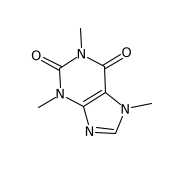
\includegraphics[scale=0.7]{imagenes/caffeine.png}}  
    \caption{Fórmula orgánica de la cafeína} \label{fig:figura1}
\end{figure}

\noindent En ellas aparecen principalmente tres elementos:

\begin{itemize}
    \item \textbf{Átomos:} Se sitúan en los extremos de los enlaces. Representados con letras que indican el elemento químico del que se trata. En caso de no existir letra, es porque estamos ante un átomo de carbono.
    \item \textbf{Enlaces:} Unen distintos átomos
    \item \textbf{Cargas:} 
\end{itemize}